\documentclass[11pt,tikz,border=0pt]{standalone}
\usepackage[T1]{fontenc}
\usepackage{newpxtext,amsmath,newpxmath,graphicx}
\usetikzlibrary{arrows.meta}
\begin{document}
\begin{tikzpicture}[x=1mm,y=-1mm]
\path[use as bounding box] (0,0) rectangle (125,82);
\node[anchor=north west,inner sep=0] at (0,0) {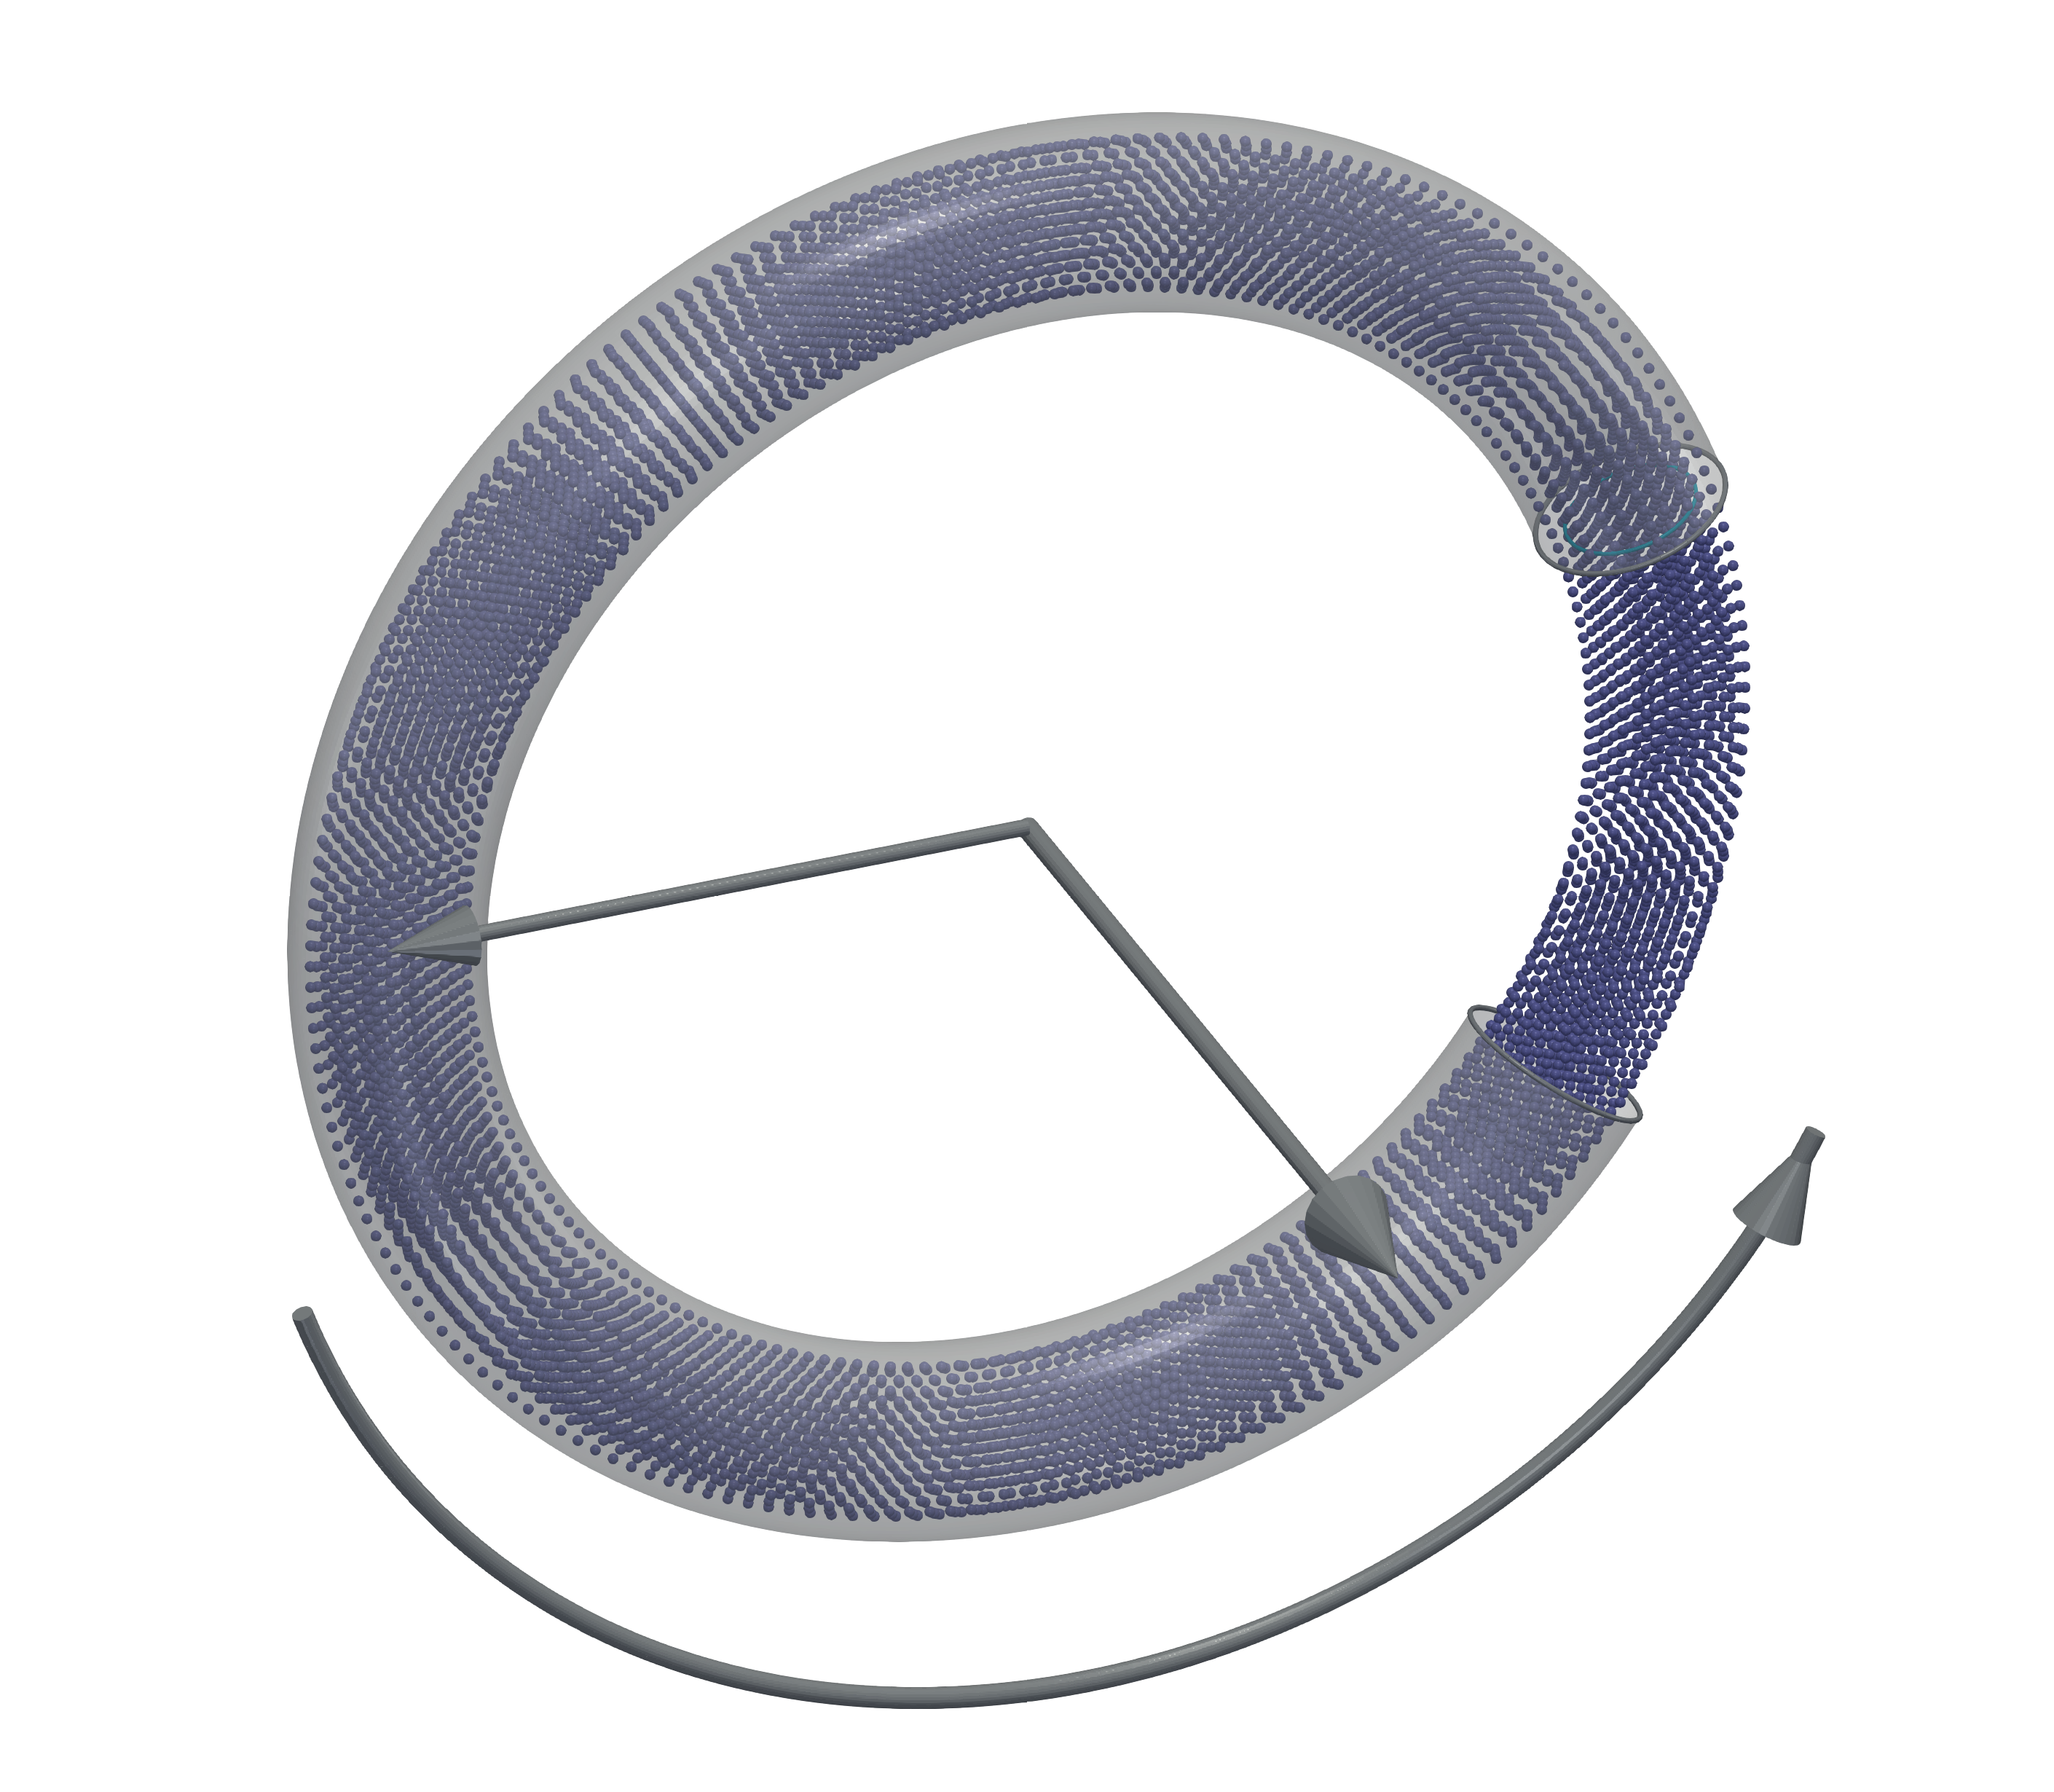
\includegraphics[width=94mm,height=82mm]{vortex_ring_schematic.png}};
\node[anchor=north west,inner sep=0] at (90,8) {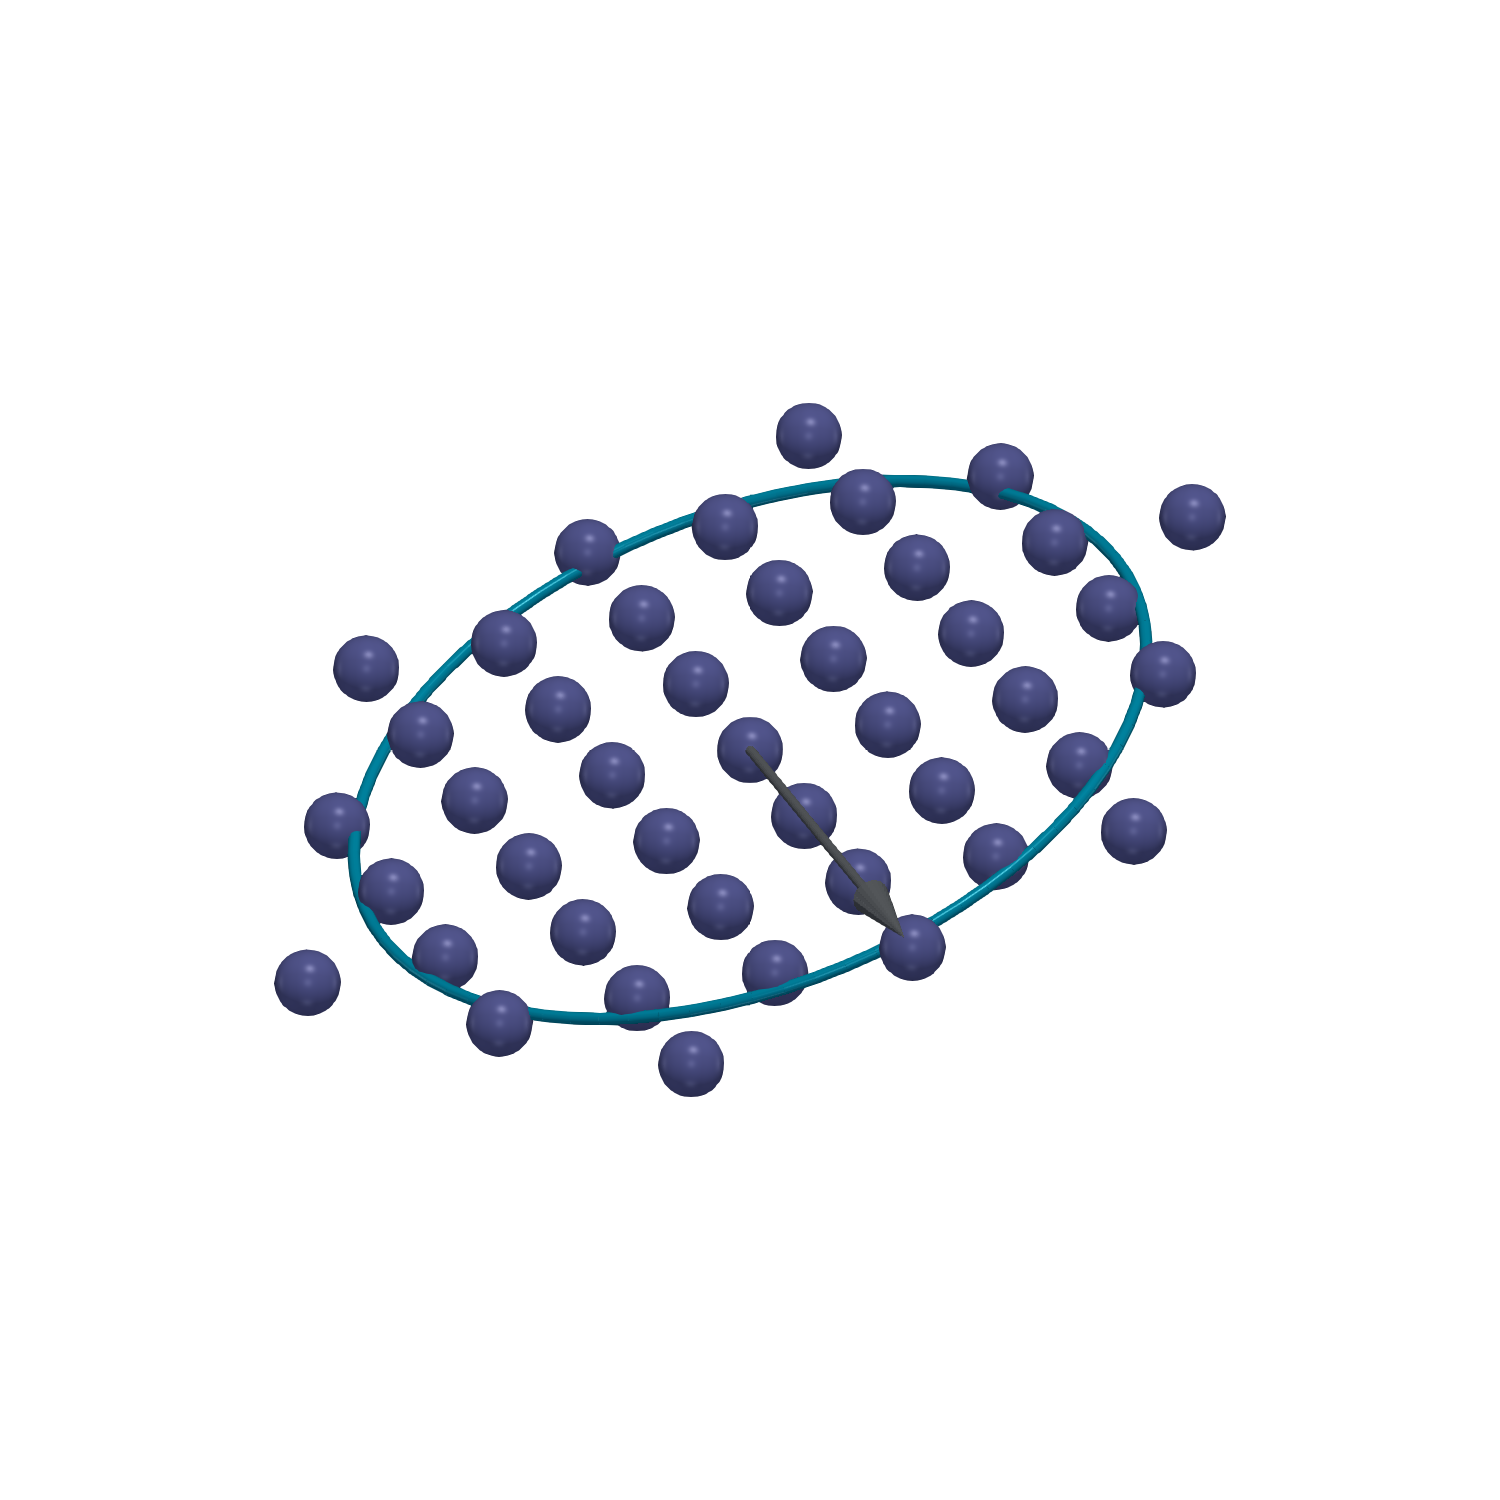
\includegraphics[width=35mm]{vortex_ring_core_detail.png}};
\node at (29,36) {$R_0$};
\node at (44,54) {$U_{\mathrm{ring}}\,\boldsymbol{e}_x$};
\node at (85,61) {$\boldsymbol{\omega}$};
\node[anchor=north] at (107.5,2) {Core section};
\node at (117,32) {$a_0$};
\node[align=center] at (106.5,45) {$a_0/R_0=0.10$};
\node at (106,57) {$\mathrm{Re}_\Gamma=\Gamma_0/\nu=3000$};
\draw[cyan!65!black,densely dotted,line width=.55pt] (74.618,23.313) -- (98,25.5);

\end{tikzpicture}
\end{document}
